% CORPO DO TRABALHO: os arquivos aparecem no PDF nesta ordem.
% Embora a pasta se chame capitulos, o modo article usa \section nos títulos.
% Para acrescentar uma seção, crie seu .tex e inclua outra linha \input{...}.

% Paginação em algarismos arábicos no canto superior direito, tamanho 10,
% começando na primeira folha da parte textual (manual IFPI 2024, seção 3.5).
% O estilo abntifpi é definido em abntex-ifpi/abntex-ifpi.sty.
\pagestyle{abntifpi}

% INTRODUÇÃO: substitua as orientações pelo texto da sua pesquisa.
% Preserve o identificador do \label se ele for citado em outras seções.
\section{Introdução}
\label{sec:introducao}

Apresente o tema e delimite o problema que será investigado. Explique por que
o estudo é relevante, formule a pergunta de pesquisa e indique o objetivo
geral e os objetivos específicos. Situe o leitor no contexto do trabalho.

Este modelo contém textos, imagens e referências de demonstração. Substitua-os
pelos materiais da sua pesquisa antes da entrega. A aparência do documento é
controlada pelos arquivos de configuração; não ajuste cada parágrafo manualmente.

% Exemplo de citação: a chave identifica uma entrada em bibliografia.bib.
Uma citação entre parênteses é produzida assim: \cite{SilvaNeto2019Credibility}.
Este exemplo demonstra o comando, não estabelece uma relação entre a obra
citada e o tema que você escolher.

% Tabela com largura ajustável: X ocupa o espaço que sobra na linha.
A \autoref{tab:identificador} demonstra uma tabela com quatro colunas.

\begin{table}[htb]
  \centering
  \ABNTEXfontereduzida
  \caption{Exemplo de organização de informações}
  \label{tab:identificador}
  \begin{tabularx}{\linewidth}{lllX}
    \toprule
    \textbf{Item} & \textbf{Categoria} & \textbf{Etapa} & \textbf{Descrição} \\
    \midrule
    1 & Exemplo & Inicial & Substitua este conteúdo pelos dados do trabalho.
    A última coluna ajusta sua largura automaticamente. \\
    \bottomrule
  \end{tabularx}
  \fonte{Elaboração própria; dados fictícios para demonstração.}
\end{table}

% Atualize este parágrafo caso acrescente ou remova seções.
O trabalho está organizado em introdução (Seção~\ref{sec:introducao}),
fundamentação teórica (Seção~\ref{sec:fundamentacao}), metodologia
(Seção~\ref{sec:metodologia}), resultados e discussão
(Seção~\ref{sec:resultados-discussoes}) e conclusão
(Seção~\ref{sec:conclusao}).

% FUNDAMENTAÇÃO: apresente os conceitos e as pesquisas relacionados ao tema.
\section{Fundamentação Teórica}
\label{sec:fundamentacao}

Defina os conceitos necessários à compreensão da pesquisa. Organize a revisão
por assuntos, compare as contribuições dos autores e identifique a lacuna que
seu trabalho pretende investigar. Cite as fontes efetivamente consultadas.

\subsection{Citações e referências}

% \citeonline insere o nome do autor na frase; \cite usa parênteses.
Exemplo do comando de citação no corpo da frase:
\citeonline{SilvaNeto2019Credibility}. Exemplo entre parênteses:
\cite{SilvaNeto2019Credibility}. Os dados são recuperados automaticamente
do arquivo de bibliografia.

\subsubsection{Citação em bloco}

O ambiente a seguir demonstra a formatação de uma citação longa. O conteúdo
é uma instrução de preenchimento, não uma transcrição de uma obra publicada.

\begin{citacao}
  Substitua este parágrafo pelo trecho exato da obra consultada. Identifique
  a autoria e a localização do trecho na fonte. Não mantenha este texto de
  orientação como se fosse uma citação real. Confira a transcrição e os
  requisitos de apresentação adotados pelo seu curso antes da entrega.
\end{citacao}

% Para indicar uma página real, use \cite[p.~número]{chave-da-obra}.
Não digite a lista de referências manualmente: ela é produzida a partir das
citações presentes no documento. As referências antigas mantidas no banco
de exemplos não representam uma verificação das normas em vigor.

% EXEMPLO -- as duas figuras abaixo vieram do modelo original e não têm
% relação com o seu tema. Troque as imagens, as legendas e as fontes.
\subsection{Exemplos de gráficos}

As Figuras~\ref{graf1} e~\ref{graf2} demonstram a inclusão de imagens.
Troque os arquivos, os títulos e as fontes pelos materiais da sua pesquisa.
A numeração é automática; não escreva o número dentro da legenda.

\begin{figure}[htb]
  \centering
  \caption{Atendimento na educação básica por dependência administrativa
  no município de Avaré, 2014}
  \label{graf1}
  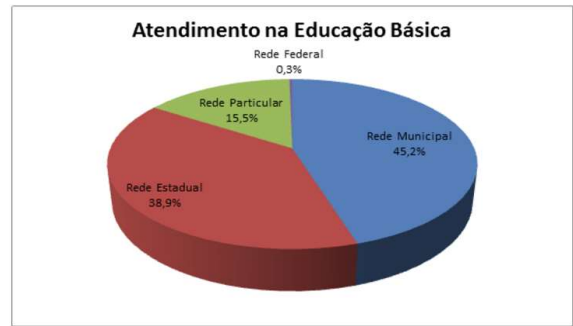
\includegraphics[width=0.85\linewidth]{imagens/grafs_1.png}
  \fonte{Secretaria Municipal de Educação de Avaré (2014), conforme o exemplo original.}
\end{figure}

\begin{figure}[htb]
  \centering
  \caption{Distribuição do número de matrículas por etapas da educação básica
  no município de Avaré, 2014}
  \label{graf2}
  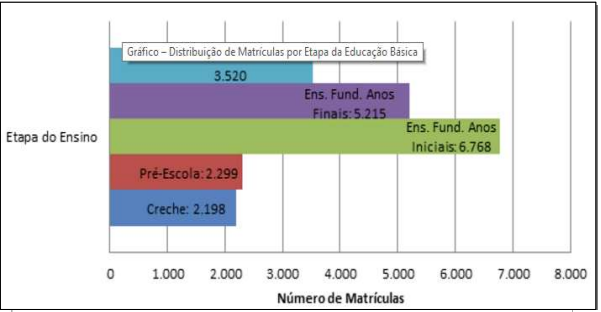
\includegraphics[width=0.85\linewidth]{imagens/grafs_2.png}
  \fonte{Secretaria Municipal de Educação de Avaré (2014), conforme o exemplo original.}
\end{figure}

% EXEMPLO -- figura de demonstração; confira a procedência antes de reusar.
\subsection{Exemplo de ilustração}

A \autoref{fig_arranjo} demonstra uma imagem acompanhada de uma citação na
indicação de fonte. Discuta no texto o que cada figura acrescenta à pesquisa,
em vez de apenas inseri-la.

\begin{figure}[htb]
  \centering
  \caption{Arranjo produtivo local da banana orgânica}
  \label{fig_arranjo}
  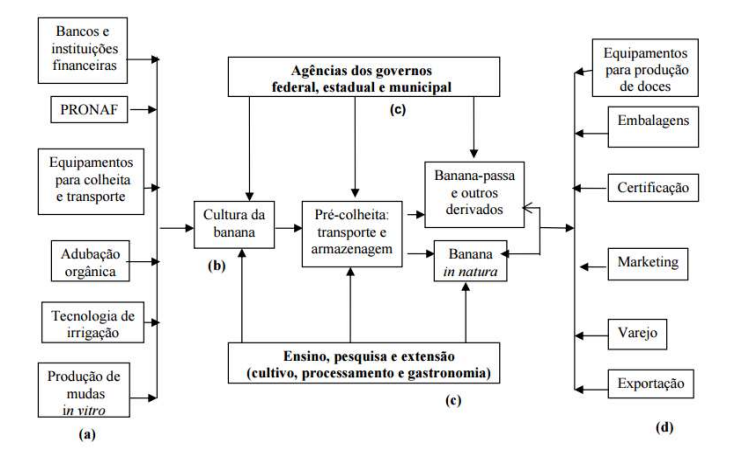
\includegraphics[width=0.8\linewidth]{imagens/fig_exemplo.png}
  \fonte{\citeonline{limaarranjo}.}
\end{figure}

% METODOLOGIA: descreva como a pesquisa foi realizada, não apenas sua finalidade.
\section{Metodologia}
\label{sec:metodologia}

Descreva o tipo de pesquisa, o contexto, os materiais ou participantes, os
critérios de seleção, os instrumentos de coleta e os procedimentos de análise.
Forneça detalhes suficientes para que o leitor compreenda as etapas realizadas.
Quando aplicável, apresente os cuidados éticos e as limitações do método.

Uma explicação complementar pode ser inserida em nota de rodapé\footnote{Este
é um exemplo de nota. Substitua-o por uma informação relevante ou remova-o.}.

% EXEMPLO -- a tabela abaixo é conteúdo de demonstração do modelo original.
\subsection{Exemplo de tabela com texto}

A \autoref{tab-nivinv} ilustra uma tabela com células de texto e largura
ajustada à página. O conteúdo é um exemplo herdado do modelo original.

\begin{table}[htb]
  \centering
  \caption{Níveis de investigação}
  \label{tab-nivinv}
  {\ABNTEXfontereduzida
  \begin{tabularx}{\linewidth}{>{\raggedright\arraybackslash}X
    >{\raggedright\arraybackslash}X
    >{\raggedright\arraybackslash}X
    >{\raggedright\arraybackslash}X}
    \toprule
    \textbf{Nível} & \textbf{Insumos} & \textbf{Sistema de investigação} & \textbf{Produtos} \\
    \midrule
    Metanível & Filosofia da ciência & Epistemologia & Paradigma \\
    Nível do objeto & Paradigmas do metanível e evidências do nível inferior
      & Ciência & Teorias e modelos \\
    Nível inferior & Modelos, métodos e problemas & Prática & Solução de problemas \\
    \bottomrule
  \end{tabularx}}
  \fonte{\citeonline{van86}.}
\end{table}

\subsection{Exemplo de quadro}

Tabela e quadro não são a mesma coisa. A tabela apresenta dado numérico
como informação central e tem as laterais abertas; o quadro é fechado em
todos os lados e apresenta dados qualitativos. O
Quadro~\ref{quad:instrumentos} demonstra o ambiente próprio para quadros,
que tem numeração e lista independentes das tabelas.

\begin{quadro}[htb]
  \centering
  \caption{Instrumentos de coleta por etapa: exemplo fictício}
  \label{quad:instrumentos}
  {\ABNTEXfontereduzida
  \begin{tabularx}{\linewidth}{|l|X|}
    \hline
    \textbf{Etapa} & \textbf{Instrumento} \\
    \hline
    Diagnóstico & Questionário aplicado aos participantes. \\
    \hline
    Avaliação & Roteiro de entrevista semiestruturada. \\
    \hline
  \end{tabularx}}
  \fonte{Elaboração própria.}
\end{quadro}

\subsection{Exemplo de tabela com números}

A \autoref{tabela-ibge} usa o comando de formatação de tabelas do modelo,
com indicação da fonte e uma nota. Os valores são fictícios.

\begin{table}[htb]
  \centering
  \IBGEtab{%
    \caption{Participantes por etapa: exemplo fictício}
    \label{tabela-ibge}
  }{%
    \begin{tabular}{lrr}
      \toprule
      \textbf{Etapa} & \textbf{Convidados} & \textbf{Participantes} \\
      \midrule
      Inicial & 30 & 24 \\
      Final & 24 & 20 \\
      \bottomrule
    \end{tabular}
  }{%
    \fonte{Elaboração própria.}
    \nota{Valores usados somente para demonstrar a formatação.}
  }
\end{table}

% RESULTADOS: substitua os exemplos e interprete os dados obtidos na pesquisa.
\section{Resultados e Discussão}
\label{sec:resultados-discussoes}

Apresente os resultados de acordo com os objetivos do trabalho. Explique as
tendências observadas, compare-as com a literatura e discuta limitações e
possíveis interpretações. Diferencie resultados medidos de hipóteses e expectativas.

% EXEMPLO -- gráfico de demonstração do abnTeX2. Substitua pelo seu.
A \autoref{fig_grafico} demonstra a inclusão de um gráfico em PDF.

\begin{figure}[htb]
  \centering
  \caption{Exemplo de gráfico incluído a partir de um arquivo PDF}
  \label{fig_grafico}
  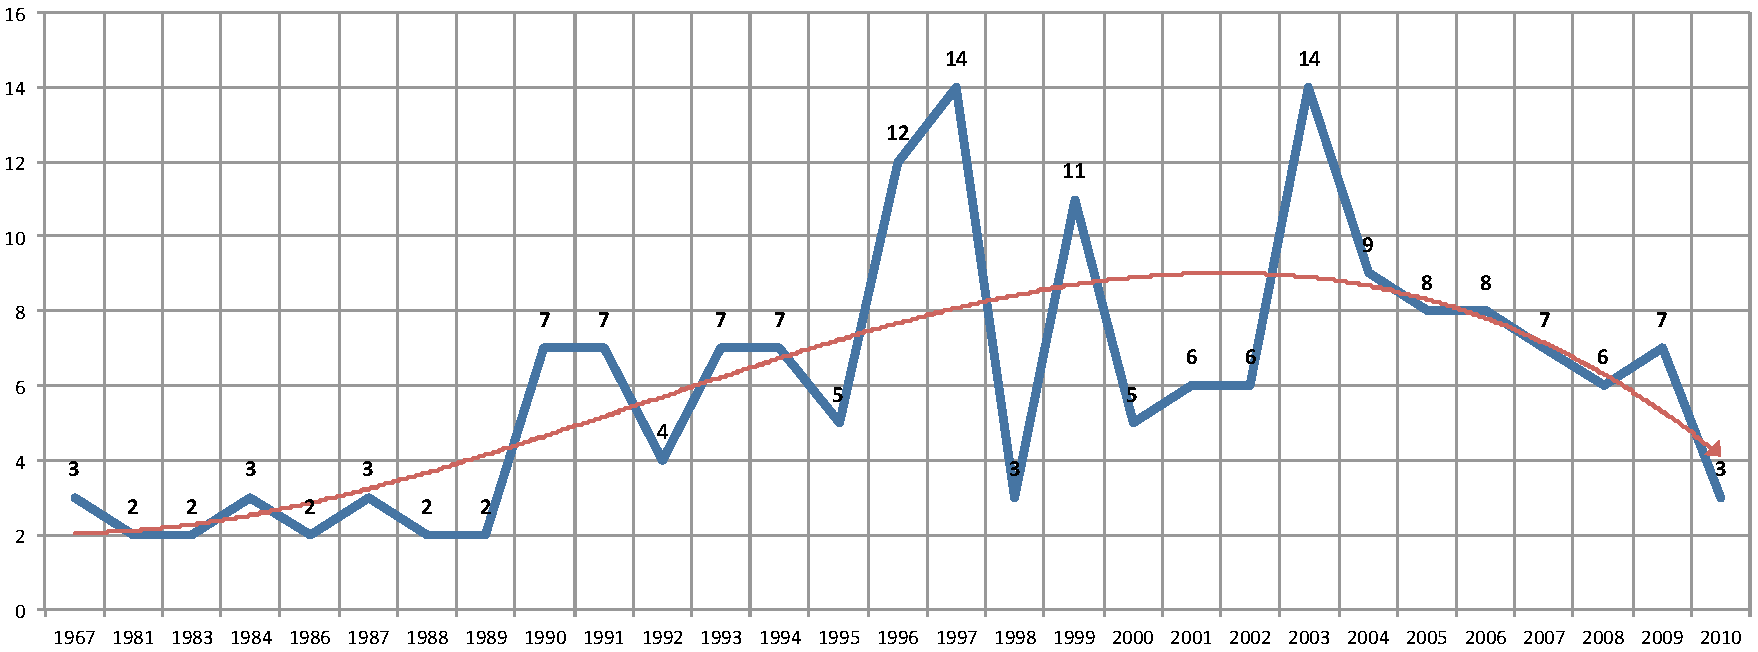
\includegraphics[width=0.7\linewidth]{imagens/abntex2-modelo-img-grafico.pdf}
  \fonte{\citeonline[p.~24]{araujo2012}.}
\end{figure}

\subsection{Equações e fórmulas}

Equações e fórmulas destacadas do parágrafo ficam centralizadas e, quando
necessário, numeradas com algarismos arábicos entre parênteses, alinhados
à direita. O ambiente \codigo{equation} faz as duas coisas; cite a equação
no texto pelo identificador, como na Equação~\ref{eq:exemplo}.

\begin{equation}
  \label{eq:exemplo}
  E = mc^{2}
\end{equation}

Se a expressão precisar ser quebrada em mais de uma linha, interrompa-a
antes do sinal de igualdade ou depois dos sinais de adição, subtração,
multiplicação e divisão.

As Figuras~\ref{fig_minipage_imagem1} e~\ref{fig_minipage_grafico2}
mostram como posicionar duas imagens lado a lado. Cada imagem tem legenda,
identificador e fonte próprios.

% Dentro de cada minipage, \linewidth corresponde à largura daquela coluna.
\begin{figure}[htb]
  \centering
  \begin{minipage}{0.46\linewidth}
    \centering
    \caption{Exemplo de imagem institucional}
    \label{fig_minipage_imagem1}
    
\includegraphics[height=2cm]{abntex-ifpi/logo_ifpi.pdf}
    \fonte{IFPI; arquivo fornecido com o modelo.}
  \end{minipage}
  \hfill
  \begin{minipage}{0.46\linewidth}
    \centering
    \caption{Exemplo de gráfico na segunda coluna}
    \label{fig_minipage_grafico2}
    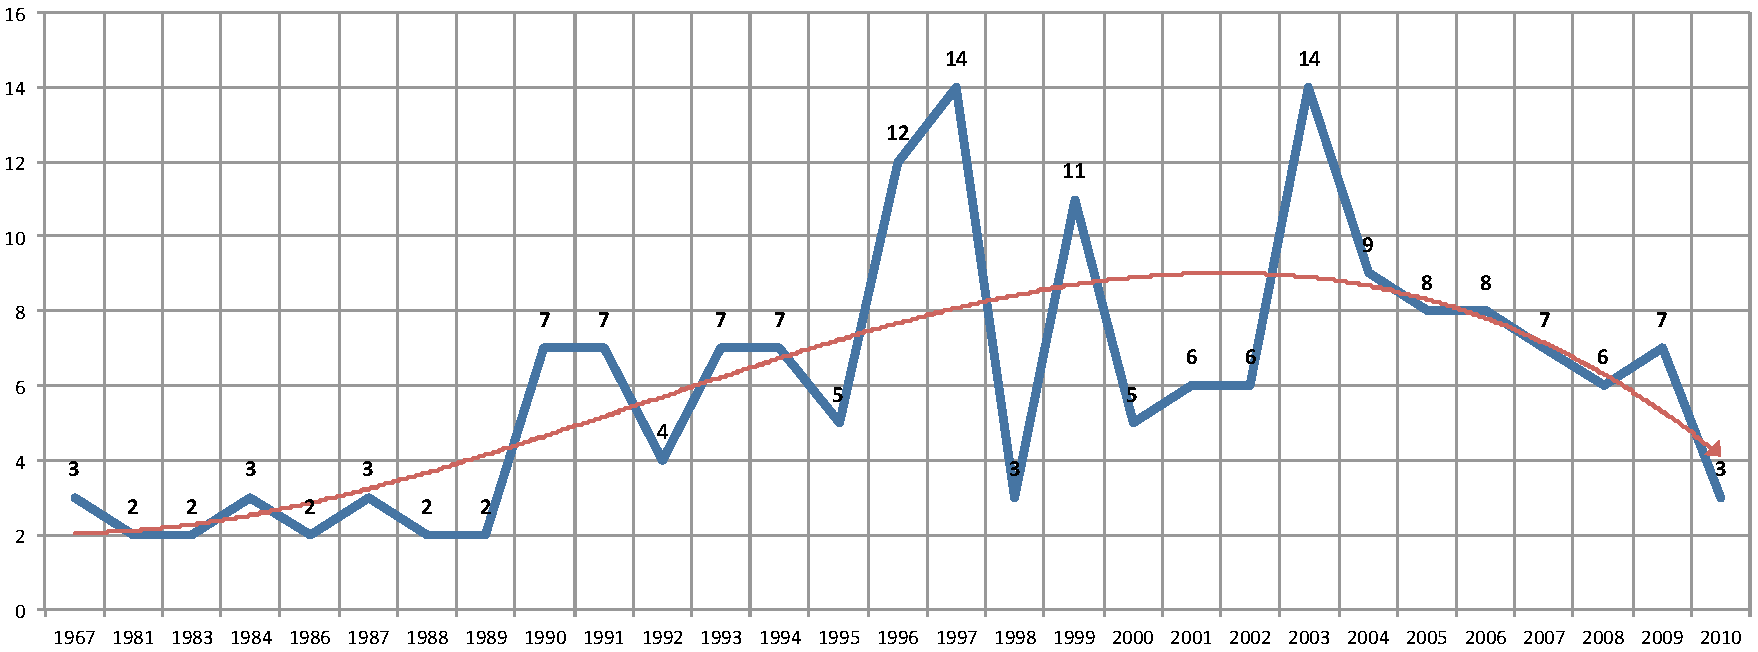
\includegraphics[width=\linewidth]{imagens/abntex2-modelo-img-grafico.pdf}
    \fonte{\citeonline[p.~24]{araujo2012}.}
  \end{minipage}
\end{figure}

% CONCLUSÃO: retome a pergunta de pesquisa e os objetivos apresentados.
\section{Conclusão}
\label{sec:conclusao}

Sintetize as principais contribuições do trabalho e indique em que medida
os objetivos foram alcançados. Responda à pergunta de pesquisa com base nos
resultados apresentados. Reconheça as limitações do estudo e evite introduzir
dados novos que não tenham sido discutidos anteriormente.

% A subseção de trabalhos futuros está em 06-trabalhos-futuros.tex.

% ----------------------------------------------------------
% Trabalhos Futuros
% ----------------------------------------------------------

% Esta subseção pertence à conclusão, apesar de ficar em arquivo separado.
% Para torná-la uma seção independente, troque \subsection por \section.
\subsection{Trabalhos Futuros}

Indique possibilidades de continuidade da pesquisa, melhorias no método ou
novas perguntas que surgiram a partir dos resultados. Relacione as propostas
às limitações identificadas no trabalho, sem apresentá-las como resultados
já obtidos.

